\documentclass[a4paper 12pt]{article}

\usepackage[utf8]{inputenc}
\usepackage[T1]{fontenc}
\usepackage{mathptmx}
\usepackage{textcomp}
\usepackage[UKenglish]{babel}
\usepackage{amsmath, amssymb}
\usepackage{float}
\usepackage{xcolor}
\definecolor{backcolor}{rgb}{0.95,0.95,0.92}
\definecolor{codegreen}{rgb}{0,0.6,0}
\definecolor{codepurple}{rgb}{0.58,0,0.82}
\usepackage{listings}
\lstdefinestyle{code}{
	backgroundcolor=\color{backcolor},
	commentstyle=\color{codegreen},
	keywordstyle=\color{magenta},
	stringstyle=\color{codepurple},
	frame=single,
	captionpos=b,
	showspaces=false,
	showstringspaces=false,
	breaklines=true,
}
\lstset{style=code}
\usepackage[hidelinks]{hyperref}
\hypersetup{
	colorlinks=false
}
\usepackage[style=ieee]{biblatex}
\bibliography{sources/biblio}
\renewcommand{\baselinestretch}{1.5}

\setlength{\parindent}{0pt}
\setlength{\parskip}{1em}

% figure support
\usepackage{import}
\usepackage{xifthen}
\pdfminorversion=7
\usepackage{pdfpages}
\usepackage{transparent}
\newcommand{\incfig}[1]{%
	\def\svgwidth{\columnwidth}
	\import{./figures/}{#1.pdf_tex}
}

\pdfsuppresswarningpagegroup=1

\begin{document}
\hypersetup{pageanchor=false}
\begin{titlepage}
  \begin{center}

    \textsc{\LARGE Dublin City University}\\[1cm]
    \textsc{\Large Electronic and Computer Engineering}\\[0.5cm]

    {\LARGE \bfseries An Evaluation of Distributed Denial of Service Attacks in
    IoT Networks\\[0.4cm]}
    {\Large \bfseries Project Design Plan\\[0.4cm]}

    \begin{figure}[H]
	
\includegraphics{images/Dcu-logo.png}
	\centering
    \end{figure}

    \vskip 2cm
    \emph{Author}\\[0.1cm]
    \noindent\makebox[\textwidth]{%
      \begin{tabular}{ll}%
        Michael Lenehan & michael.lenehan4@mail.dcu.ie \\
	Student Number: & 15410402 \\
    \end{tabular}}\\[0.1cm]

    \vfill

    % Bottom of the page
    % Probably replaced with date of deadline
    {\large{15/06/2020}}

  \end{center}
\end{titlepage}

\hypersetup{pageanchor=true}
\pagenumbering{alph}
\thispagestyle{plain}
\begingroup
\renewcommand{\cleardoublepage}{}
\renewcommand{\clearpage}{}

\LARGE{Declaration}

\endgroup

\vskip 1cm

I declare that this material, which I now submit for assessment, is entirely my
own work and has not been taken from the work of others, save and to the extent
that such work has been cited and acknowledged within the text of my work. I
understand that plagiarism, collusion, and copying are grave and serious
offences in the university and accept the penalties that would be imposed should
I engage in plagiarism, collusion or copying. I have read and understood the
Assignment Regulations set out in the module documentation. I have identified
and included the source of all facts, ideas, opinions, and viewpoints of others
in the assignment references. Direct quotations from books, journal articles,
internet sources, module text, or any other source whatsoever are acknowledged
and the source cited are identified in the assignment references. This
assignment, or any part of it, has not been previously submitted by me or any
other person for assessment on this or any other course of study.

I have read and understood the DCU Academic Integrity and Plagiarism at
\url{https://www4.dcu.ie/sites/default/files/policy/1%20-%20integrity_and_plagiarism\_ovpaa_v3.pdf}
and IEEE referencing guidelines found at
\url{https://loop.dcu.ie/mod/url/view.php?id=448779}.

\vskip 1cm
Signed: \underline{\ \ \ \ \ \ \ \ \ \ \ \ \ \ \ \ \ \ \ \ \ \ \ \ \ \ \ \ \ \ \
\ \ \ \ \ \ } \hspace{20mm}Date: \underline{15/06/2020}

\hspace*{0mm}\phantom{Signed:}Michael Lenehan

\pagebreak

\pagenumbering{arabic}
\tableofcontents
\clearpage
\section{Research Question}
This project aims to critically and technically evaluate the susceptibility of
IoT networks to DDoS attacks, focusing on the devices, networks, and operating
systems associated with IoT.

\section{Project Scope}
The following list describes the topics and technologies which will be utilized
in the completion of this project.

\begin{itemize}
	\item Susceptibility to Attack
	\begin{itemize}
		\item Networks
		\begin{itemize}
			\item ns-3 Network Simulations
		\end{itemize}
		\item Operating Systems
		\begin{itemize}
			\item OS Level Security Feature Implementations
			\item Known
		\end{itemize}
	\end{itemize}
	\item Mitigation/Detection
\end{itemize}

\section{Design Approach}
The proposed approach to this project is to present a detailed technical
evaluation of the security features available at the operating systems
level. These will include features such as networking security - i.e.
firewalls, and software security - i.e. secure boot.

Simulations will be run using ns-3 in order to evaluate the effects of
common DDoS attacks on networks consisting of IoT devices. These simulations
will utilize the available IoT related protocols in ns-3, including IPv6 and
6LoWPAN. The results of these simulations will be evaluated to determine points
of failure within the networks.

Finally, a technical evaluation will be done into the available detection and
mitigation techniques. This will include recommendations of techniques which
could have specific benefits in IoT networks.

\section{Timeline}
The Gannt chart below describes the proposed timeline for the project. All items
within the Gannt chart are colour coded as follows; green represents
documentation - i.e. work on the final report, red represents background
research - i.e. background research required for understanding the topic, blue
represents testing - i.e. simulation testing, orange represents end of week
reviews, during which time the goals of the past week and following week will be
assessed.

\begin{figure}[H]
	\centering
	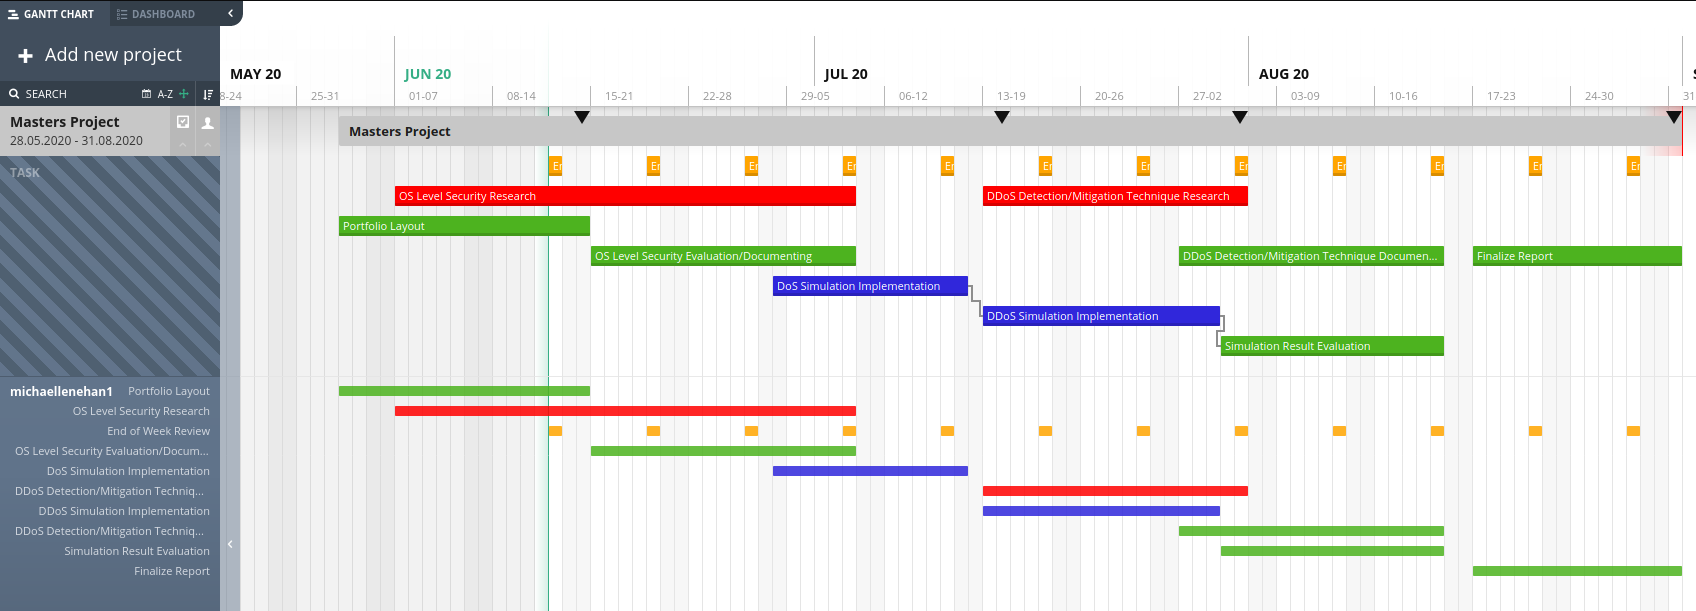
\includegraphics[width=\textwidth]{images/GanntChart}
	\caption{Project Gannt Chart}
	\label{fig:images-GanntChart}
\end{figure}

This project plan can be viewed at the following link:
\url{https://app.agantty.com/#/sharing/d595b7c64d314f5788834d0ed8614ccc/de}

Not included in this design plan are working hours, which, for the duration of
the project, will be 8 a.m. to 5 p.m Monday to Friday. All project work must be completed outside
of these times.

\section{Success Criteria}
This project will be considered successful if the following criteria are met:

\begin{enumerate}
	\item The completion of a literature review
	\item The completion of a project project presentation
	\item The completion of a Masters project research log
	\item The completion of a technical evaluation of OS level
		security implementations
	\item The completion of an investigation into known security
		vulnerabilities of IoT operating systems
	\item The completion of a number of DDoS simulations on simulated IoT
		networks
	\item The completion of a technical evaluation of DDoS detection and
		mitigation techniques
	\item The completion of a list of recommendations of
		detection/mitigation techniques specifically applicable to IoT
		networks.
\end{enumerate}

\section{Remote Arrangements}
It has been confirmed with the project supervisor, Liam Meany, that this project
can be successfully completed remotely, i.e. with no access to on-campus
resources.

\end{document}
